% Paste into IEEE LaTeX (adjust path if needed)
\subsection{NDN Forwarder Proof-of-Concept}
Separate from the IP-validated R18 cascade, we simulate a single NDN router
with Pending Interest Table (PIT) and Content Store (CS), reproducing
\textsc{Interest Flooding} and \textsc{Cache Pollution} attacks.
A Random Forest on 20-packet windows of 17 NDN-native features achieves
0.9953 macro-F1 on 51,656 held-out windows (99.65\% attack detection, 0.67\% benign FPR).

\begin{figure}[!t]
\centering
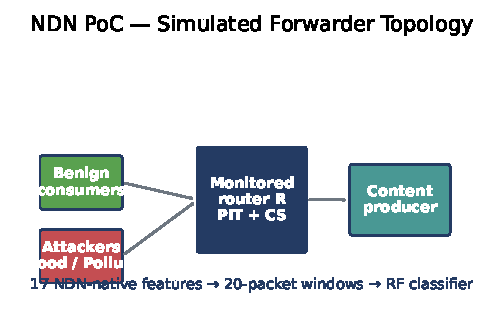
\includegraphics[width=\linewidth]{docs/ndn_poc/ieee/fig_ndn_architecture.pdf}
\caption{NDN PoC simulation topology (PIT + Content Store).}
\label{fig:ndn_arch}
\end{figure}

\begin{figure}[!t]
\centering
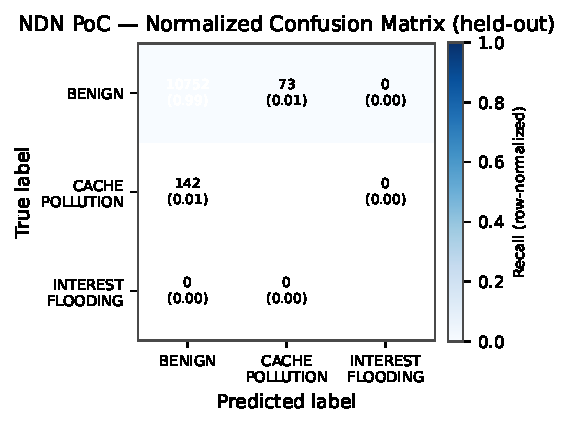
\includegraphics[width=0.48\linewidth]{docs/ndn_poc/ieee/fig_ndn_confusion_matrix.pdf}
\hfill
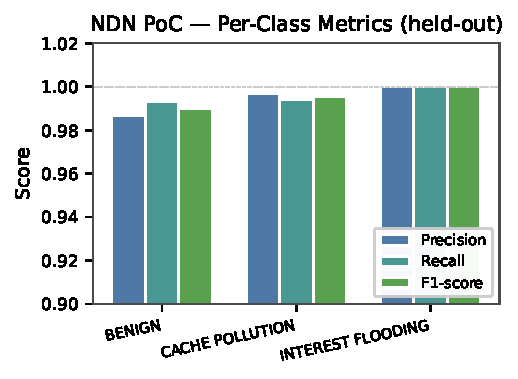
\includegraphics[width=0.48\linewidth]{docs/ndn_poc/ieee/fig_ndn_per_class_metrics.pdf}
\caption{NDN PoC held-out results: normalized confusion matrix (left) and per-class metrics (right).}
\label{fig:ndn_results}
\end{figure}

\begin{figure}[!t]
\centering
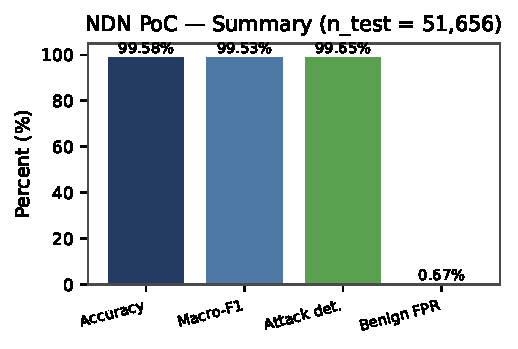
\includegraphics[width=0.75\linewidth]{docs/ndn_poc/ieee/fig_ndn_summary_metrics.pdf}
\caption{NDN PoC summary metrics on held-out test windows.}
\label{fig:ndn_summary}
\end{figure}
